%%% template.tex
%%%
%%% This LaTeX source document can be used as the basis for your technical
%%% paper or abstract. Intentionally stripped of annotation, the parameters
%%% and commands should be adjusted for your particular paper - title, 
%%% author, article DOI, etc.
%%% The accompanying ``template.annotated.tex'' provides copious annotation
%%% for the commands and parameters found in the source document. (The code
%%% is identical in ``template.tex'' and ``template.annotated.tex.'')

\documentclass[conference]{acmsiggraph}

\usepackage[usenames,dvipsnames]{color}
\newcommand\memo[1]{{\color{CornflowerBlue}#1}}
\newcommand\devin[1]{{\color{BurntOrange}#1}}
\newcommand\julien[1]{{\color{RubineRed}#1}}
\newcommand\claudia[1]{{\color{Purple}#1}}
\newcommand\panayiotis[1]{{\color{Green}#1}}
\newcommand\note[1]{{\color{Red}#1}}

\usepackage{amsfonts}
\usepackage{amssymb}
\usepackage{graphicx}
\usepackage{url}
%\usepackage[tight,footnotesize]{subfigure}
%\usepackage{algorithm}
%\usepackage{algorithmic}


\TOGonlineid{45678}
\TOGvolume{0}
\TOGnumber{0}
\TOGarticleDOI{1111111.2222222}
\TOGprojectURL{}
\TOGvideoURL{}
\TOGdataURL{}
\TOGcodeURL{}

\title{Optimization-based computation of locomotion trajectories for Crowd Patches}

\author{Authors\thanks{e-mail:emails@emailplace}\\Institution}
\pdfauthor{Authors}

\keywords{keywords go here}

\begin{document}

%% \teaser{
%%   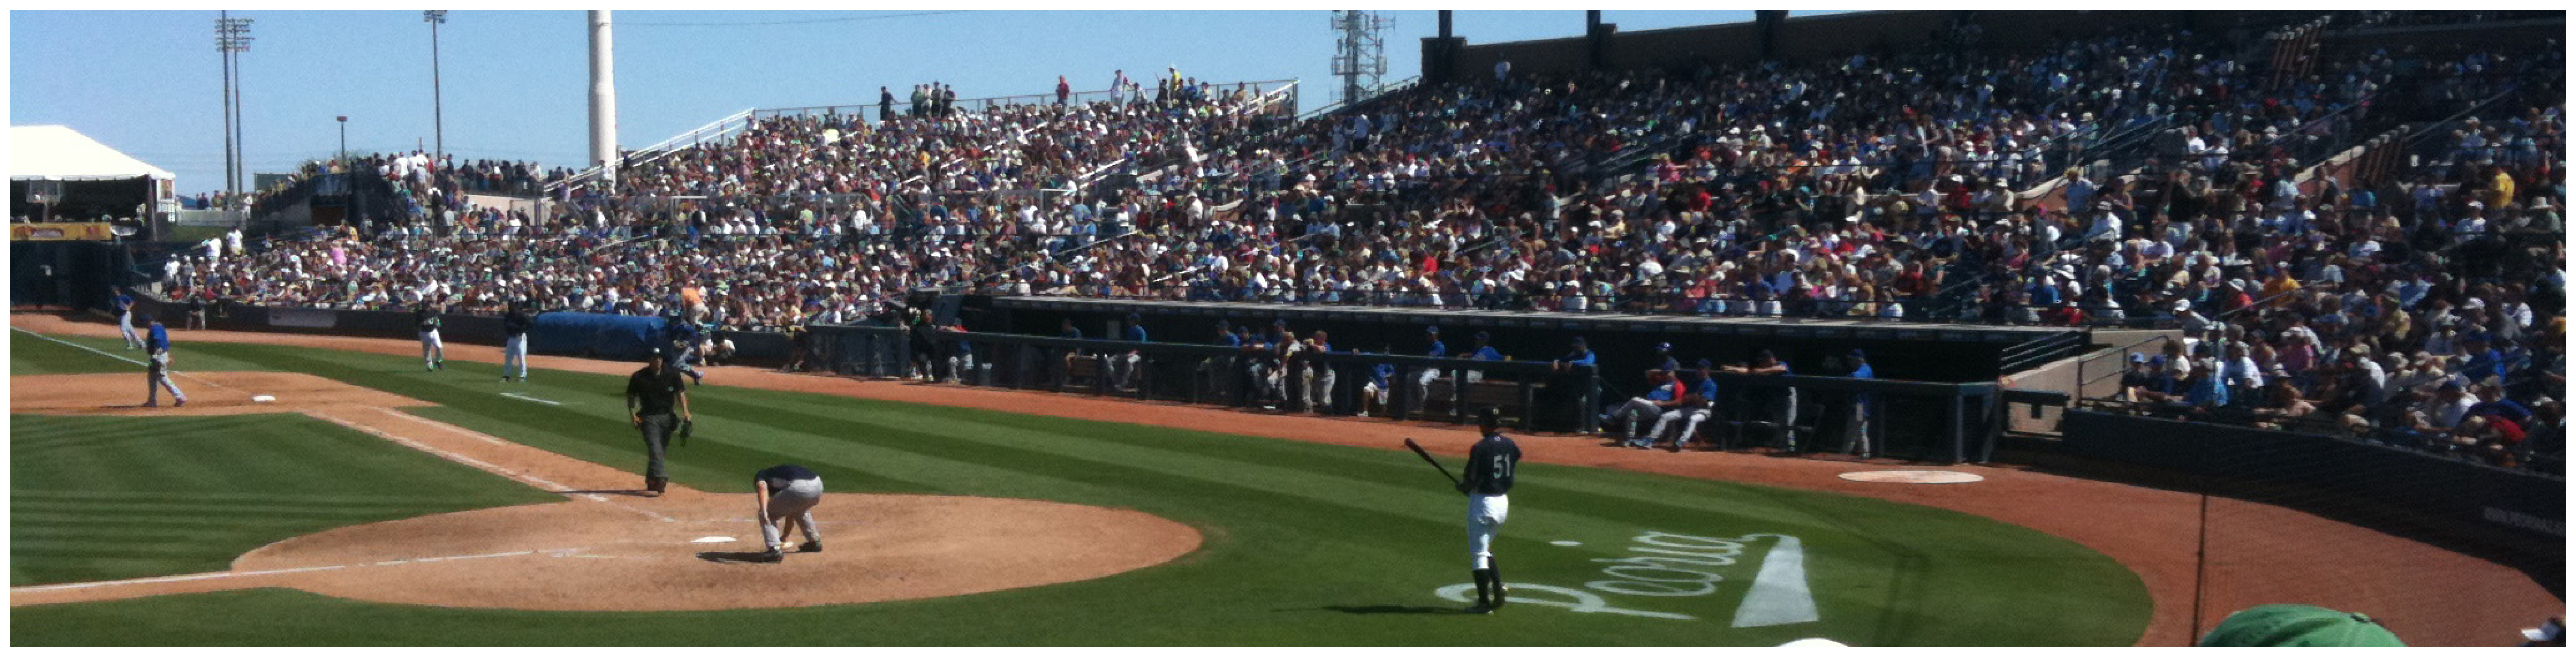
\includegraphics[height=1.5in]{images/sampleteaser}
%%   \caption{Spring Training 2009, Peoria, AZ.}
%% }

\maketitle

\begin{abstract}

Abstract, abstract, abstract ...

%Citations can be done this way~\cite{Jobs95} or this more concise way~\shortcite{Jobs95}, depending upon the application.

\end{abstract}

\begin{CRcatlist}
%  \CRcat{I.3.3}{Computer Graphics}{Three-Dimensional Graphics and Realism}{Display Algorithms}
  %\CRcat{I.3.7}{Computer Graphics}{Three-Dimensional Graphics and Realism}{Radiosity};
\end{CRcatlist}

\keywordlist

%% Use this only if you're preparing a technical paper to be published in the 
%% ACM 'Transactions on Graphics' journal.

\TOGlinkslist

%% Required for all content. 

\copyrightspace

\section{Introduction}

Video Games are constantly displaying larger and more lively virtual environments due to increased computational power and advanced rendering techniques. For example, the recent Grand Theft Auto (GTA) game~\cite{GTA:web} takes place in Los Santos and its surroundings, a completely virtual city. In spite of the impressive quality and liveliness of the scene, Los Santos still remain relatively sparsely populated with virtual people. The reason for this phenomenon is the large computational cost required to get an {\it ambient crowd} in such large environments. To address this issue, the technique of {\it Crowd Patches} has been recently introduced in~\cite{Yersin:2009}. 

{\it Crowd patches} are precomputed elements (patches) of crowd animations. Patches are time-periodic to be endlessly played in time. The boundary conditions of precomputed animations are accurately controlled to enable combining patches in space (i.e., characters can move from in-between patches), and compose large ambient crowds. This technique eases the process of designing an ambient crowd in an efficient way. 

One problem with this technique however, is to compute internal animation trajectories for patches, that satisfy both, time-periodicity and boundary conditions among patches. Satisfying both of these constraints is difficult, because it is equivalent to computing collision-free trajectories that exactly pass through spatio-temporal waypoints (i.e., at some exact position in time) whilst at the same time solving possibly complex situations of interactions with other agents (collision-avoidance). In addition, trajectories should look as natural as possible.

In this paper we propose a new optimization-based method to compute these internal trajectories. Our method starts by assigning linear trajectories which are easy to compute and satisfy both, periodicity and boundary conditions, but at the same time might produce collisions between characters. Then, iteratively, we optimize the trajectories to handle collisions. We try to keep the produced trajectories as close as possible to the initial guessed trajectories, to \note{minimize the magnitude of collision-avoidance maneuvers.} \panayiotis{How do we define this? Do we measure it?} \devin{I don't think we do either.}

To conclude, our main contribution is an optimization-based algorithm to compute high quality animation trajectories (2D global navigation trajectories) for individual crowd patches under constraints (expressed as a set of spatio-temporal boundary control points).

The remainder of this paper is organized as follows: Section \ref{state_of_the_art} proposes a short overview on the state of the art. Section \ref{the_method} details our technique to compute these internal trajectories. Then, in Section \ref{results} some results, together with their performance and quality analysis are shown before a brief discussion and concluding remarks. 

\section{State of the Art \label{state_of_the_art}}

Most often, virtual environments are populated based on crowd simulation approaches~\cite{ThalmannBook:2013}. An ambient crowd is generated from a large set of moving characters, mainly walking characters. Recent efforts in crowd simulation have enabled dealing with great performances ~\cite{PettreCAVW:2006,Treuille:2006}, high densities~\cite{Narain:2009} or controllable crowds~\cite{Guy:2009}. There has been a lot of effort to develop velocity-based approaches~\cite{Paris:2007,VanDenBerg:2008} which display much more smooth and realistic locomotion trajectories, especially thanks to anticipatory adaptation to avoid collisions between characters. \note{Nevertheless, \dots}

Simulation-based techniques are ideal to create an ambient crowd for large environments. Several problems are recurrent with such approaches: a) crowd simulation is computation demanding, crowd size is severly limited for interactive applications on light computers; b) simulation is based on simplistic behaviours (e.g. walk, avoid collisions, etc.), it is difficult to show diverse and rich crowds based on classical crowd simulation algorithms; c) crowd simulation is prone to animation artifacts or deadlock situations, it is impossible to guarantee animation quality. 

Example-based approaches attempt to solve the limitations on animation quality. The key idea of this approaches is that agents behave accordingly to set of existing example trajectories~\cite{Lerner:2007,Ju:2010,Charalambous:2014}. Locally, trajectories are necessarily of good quality, because they reproduce recorded ones. However, such approaches raise other difficulties: it is difficult to guarantee that the database of examples will cover all the required content, it can be difficult to control behaviors and interactions displayed by characters if the database content is not carefully selected. Finally, those approaches are also computationally demanding.

To solve both performances as well as quality issues, crowd patches were introduced in~\cite{Yersin:2009}. The key idea is to generate an ambient moving crowd from a set of interconnected patches. Each patch is a kind of 3D animated texture element, which records the trajectories of several moving characters. Trajectories are periodic in time, so that the crowd motion can be played endlessly. Trajectories boundary conditions, at the geometrical limits of patches are controlled to be able to connect together to patches, with characters moving from one patch to another. Thus, a crowd animated from a set of patches have a seamless motion, patches limit cannot be easily detected. The boundary conditions are all registered into {\it patterns}, which are sort of gates for patches with a set of spacetime input/output points. Please refer to the Yersin's paper for details. 

Nevertheless, using the crowd patches approach, it is important to work with a limited set of patters to enable easily connecting various patches. As a result, it is important to be able to compose a patch by starting from a set of patterns, and to deduce internal trajectories of patches from the set of bounday conditions set by patterns. As a result, we need to compute trajectories for characters that pass through a given set of spatiotemporal waypoints (not that we consider 2D trajectories for characters global motion here). This problem is difficult. Indeed, generally, steering techniques for characters consider spatial goals, but does not consider the time a character should reach its waypoint. Dedicated techniques are required. 

Yersin suggests using an adapted Helbing technique to compute internal trajectories~\cite{Helbing:2005}. The key idea is to connect input/output points together with linear trajectories, to model characters as particles attracted by a goal moving along one of these linear trajectories, combined with repulsion forces to avoid collision. One problem with this approach is limited density level, as well as the level of quality of trajectories: they suffer the usual drawbacks of Helbing's generated trajectories, i.e., lack of anticipation, which result into non natural local avoidance maneuvers. 

Compared to previous techniques to compute internal trajectories, we suggest formulating the problem of computing internal trajectories as an optimization problem. First, we suggest optimizing the way input and output points are connected. Especially, as waypoints are defined in space and time, we connect them trying to get some {\it good} walking speed (close to the average human walking speed). Indeed, characters moving too slow or too fast are visually evident artifacts. Second, after having connected waypoints with linear trajectories, we deform them to remove possible collisions. We do this through an iterative process trying to remove collisions with as limited as possible changes to the initial trajectories. We show improvements in the quality of results as compared to the original work by Yersin et al. 

\julien{Would be nice to add reference and comparison with the rule based techinique. } \panayiotis{Completely agree with that ... }
\claudia{I did not copied all the coments remaining in this Section. See google docs.}


\section{Method overview \label{the_method}}

\note{Overview: remind definitions on crowd patches: patch, pattern, spatiotemporal waypoints (boundary conditions: input, output, initial states // boundary conditions should be strictly enforced. Movable control points), period of time \dots}

\note{Starting Definitions:}

\begin{description}

\item[Patch - ]{A patch is a set $\{ A, \pi, D, S\}$ where $A$ is a geometrical area with a convex polygonal shape, $\pi$ the period of time of the animation, $D$ and $S$ are the sets of dynamic and static objects, respectively. These last two sets may be empty in case of an empty patch.}

\item[Static obstacles -]{Static objects are simple obstacles whose geometry is fully contained inside the patch.}

\item[Dynamic objects]{Dynamic objects are animated: they are moving in time according to a set of trajectories $T$.}

\end{description}

We define a {\bf trajectory} inside a patch as a function going from time to position, more specifically from the subset $[ 0,\pi ]$ to $A$:$ \tau:[t_1,t_2]\rightarrow A, \hspace{0.3cm} 0 \leq t_1 < t_2 \leq \pi$. We represent a trajectory as a list of control points connected by segments. 

A {\bf control point} is a point in space and time. All control points in a trajectory will either be a movable control point or a boundary control point. Boundary control points serve as entry and exit points to the patch and cannot be moved, added or deleted. Movable control points can be moved, added, or removed from the trajectory as long as they do not violate the \note{constraints of the patch, their position must be inside $A$ and the time between $t_1$ and $t_2$.} \\
\devin{-- Should we state exactly whate these constraints are here? }\\
\memo{-- Sure, I added a line for that}

A {\bf segment} is a straight line connecting two control points in a specific order. Since these are unidirectional lines in space-time, it is important to remember that they are not allowed to go backwards in time.

There are two categories of dynamic objects: endogenous agents and exogenous agents. {\bf Endogenous agents} remain inside $A$ for the total period of time $\pi$. In order to achieve periodicity for the animation, they are associated with a trajectory $\tau : [0,\pi] \leftarrow A$, such that it respects the periodicity condition: the position at the start and at the end of the animation must be the same, i.e. \mbox{$\tau (0) = \tau (\pi)$}.\\
{\bf Exogenous agents} go outside $A$. They enter the patch at time $t_{initial}$ and position $a_{initial}$, and they exit at time $t_{final}$ and position $a_{final}$. For each agent we associate a sequence of $n$ trajectories $\{ \tau_1, \tau_2, \dots, \tau_n\}$. Sequences may have only one trajectory, but some agents require additional trajectories in order to satisfy speed and time constraints. The following conditions must be respected in each sequence of trajectories associated with an exogenous agent:

\begin{itemize}

\item{$a_{initial}$ and $a_{final}$ must be points in the border of $A$. Otherwise, they couldn't be exogenous agents.}

\item{If the sequence is composed by more than one trajectory, for each two contiguous trajectories, the following must be true to ensure continuity: $\tau_i(\pi) = \tau_{i_{next}}(0)$.}

\end{itemize}

Note that the second condition implicitly implies that in sequences with multiple trajectories, each middle trajectory must be fully defined in the period of time $[0,\pi]$, while $\tau_1$ must be defined in $[t_{initial},\pi]$ and $\tau_n$ must be defined in $[0, t_{final}]$.

\begin{description}

\item[Pattern -]{If a patch is a spatio-temporal cube (or any other right prism, depending on the type of polygon used as its area}, then a pattern could be defined as one lateral side of the \note{cube (or right prism). Specifically, it is a rectangle whose base is one of the edges of the polygonal area (we define $l$ as this two dimensional vector), and its height is equal to the period. }

\end{description}


%\begin{figure*}
%\begin{center}
%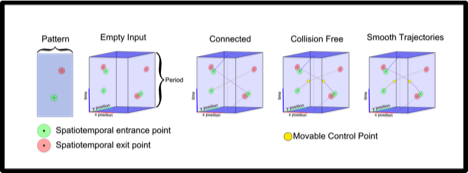
\includegraphics[width=14cm]{./images/overview.png}
%\caption{ Caption caption caption caption caption caption caption caption caption caption\label{overview}}
%\end{center}
%\end{figure*}


%\section{Results \label{results}}
%\section{Discussion}
%\section{Conclusions} 

%\begin{equation}
% \sum_{j=1}^{z} j = \frac{z(z+1)}{2}
%\end{equation}

%\begin{eqnarray}
%x & \ll & y_{1} + \cdots + y_{n} \\
%  & \leq & z
%\end{eqnarray}

%\begin{figure}[ht]
 % \centering
 % 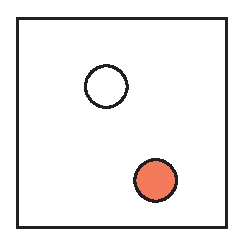
\includegraphics[width=1.5in]{images/samplefigure}
 % \caption{Sample illustration.}
%\end{figure}

%\section{Conclusion}


%\section*{Acknowledgements}

%To Robert, for all the bagels.

\bibliographystyle{acmsiggraph}
\bibliography{Crowd_Patches}
\end{document}
